%        File: experiment_EHRET_KHALIFE.tex
%     Created: Mon Feb 02 09:00 PM 2015 C
% Last Change: Mon Feb 02 09:00 PM 2015 C
%
\documentclass[a4paper]{article}
\usepackage[]{graphicx}
\author{Thibaud EHRET \& Sammy KHALIFE}
\title{Experimental report}

\begin{document}
\maketitle

In figures \ref{fig:z_5}, \ref{fig:z_42} and \ref{fig:z_105} we illustrate the law of large number for $z$ equals $5$, $42$ and $105$ respectively.

The mean for the distribution with $z$ equal $5$ is $0.1995$, $0.0238$ for $z$ equal to $42$ and $0.0095$ for $z$ equal to $105$. Each computation has been made for a number of sample of $100000$.

\begin{figure}[!Hbt]
	\centering
	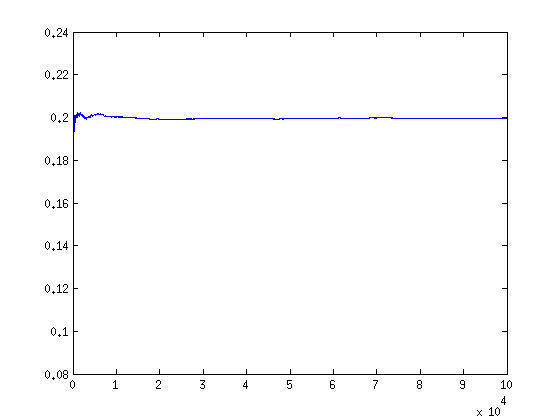
\includegraphics[scale=0.7]{z_5.png}
	\caption{Illustration of the law of large number for $z$ equal to $5$ with $100000$ samples}
	\label{fig:z_5}
\end{figure}

\begin{figure}[!Hbt]
	\centering
	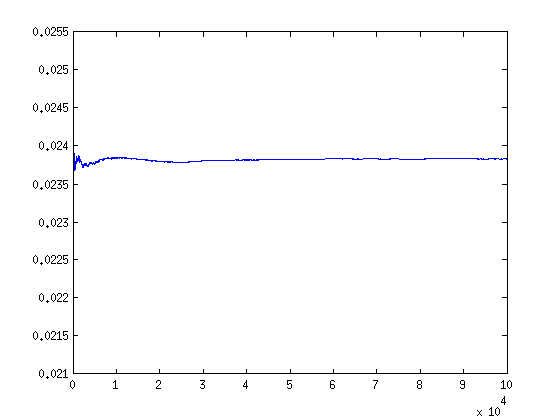
\includegraphics[scale=0.7]{z_42.png}
	\caption{Illustration of the law of large number for $z$ equal to $42$ with $100000$ samples}
	\label{fig:z_42}
\end{figure}

\begin{figure}[!Hbt]
	\centering
	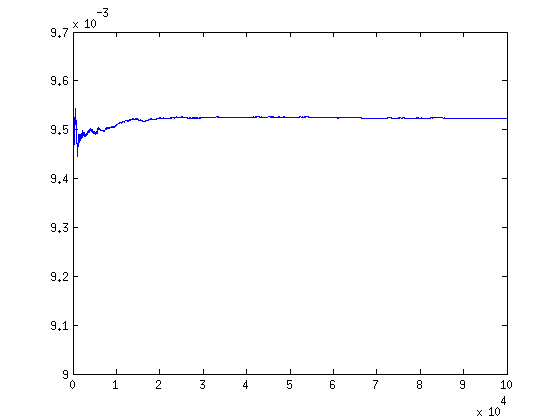
\includegraphics[scale=0.7]{z_105.png}
	\caption{Illustration of the law of large number for $z$ equal to $105$ with $100000$ samples}
	\label{fig:z_105}
\end{figure}

\end{document}


